\documentclass{article}

\usepackage{amsmath}
\usepackage{graphicx}
\usepackage{subcaption}
\usepackage{amssymb}
\usepackage{setspace}
\usepackage{tikz}
\usepackage[utf8]{inputenc}
\usepackage[english]{babel}
\usepackage{float}
\usepackage{ragged2e}
\usepackage{multicol}
\usepackage{fancyhdr}
\usepackage[export]{adjustbox}
\usepackage[margin=1in]{geometry}
\usepackage{indentfirst}
%\usepackage{color}
%\usepgflibrary{arrows}  % LATEX and plain TEX and pure pgf
%\usepgflibrary[arrows]  % ConTEXt and pure pgf
%\usetikzlibrary{arrows} % LATEX and plain TEX when using TikZ
%\usetikzlibrary[arrows] % ConTEXt when using TikZ
\usepackage{xcolor}
%\usepackage{siunitx}

%\sisetup{
%  round-mode         = places,
%  round-precision    = 3,
%}

\pagestyle{fancy}
\fancyhf{}
\chead{\textbf{Conics}}
\rhead{2021}
\lhead{Advanced Calculus 2}
\rfoot{\center \thepage}

\title{\textbf{Conics: Circles and Ellipses}}
\author{Julia Tang}
\date{January 8, 2021}

\setlength{\parindent}{3em}
\setlength{\parskip}{1em}
\setlength{\columnsep}{1cm}

\colorlet{yellowOrange}{white!50!yellow!70!orange}
\colorlet{redOrange}{orange!50!red}
\colorlet{blueGreen1}{blue!50!green}
\colorlet{blueGreen2}{blue!80!green}
\newcommand{\highlight}[1]{%
  \colorbox{yellowOrange}{$\displaystyle#1$}}

\newenvironment{question}
  {\begin{center}
  \begin{tabular}{|p{0.9\textwidth}|}
  \hline\\
  }
  {
  \\\\\hline
  \end{tabular}
  \end{center}
  }

\begin{document}

\pagenumbering{arabic}


\maketitle
\begin{figure}[H]
  \begin{center}
    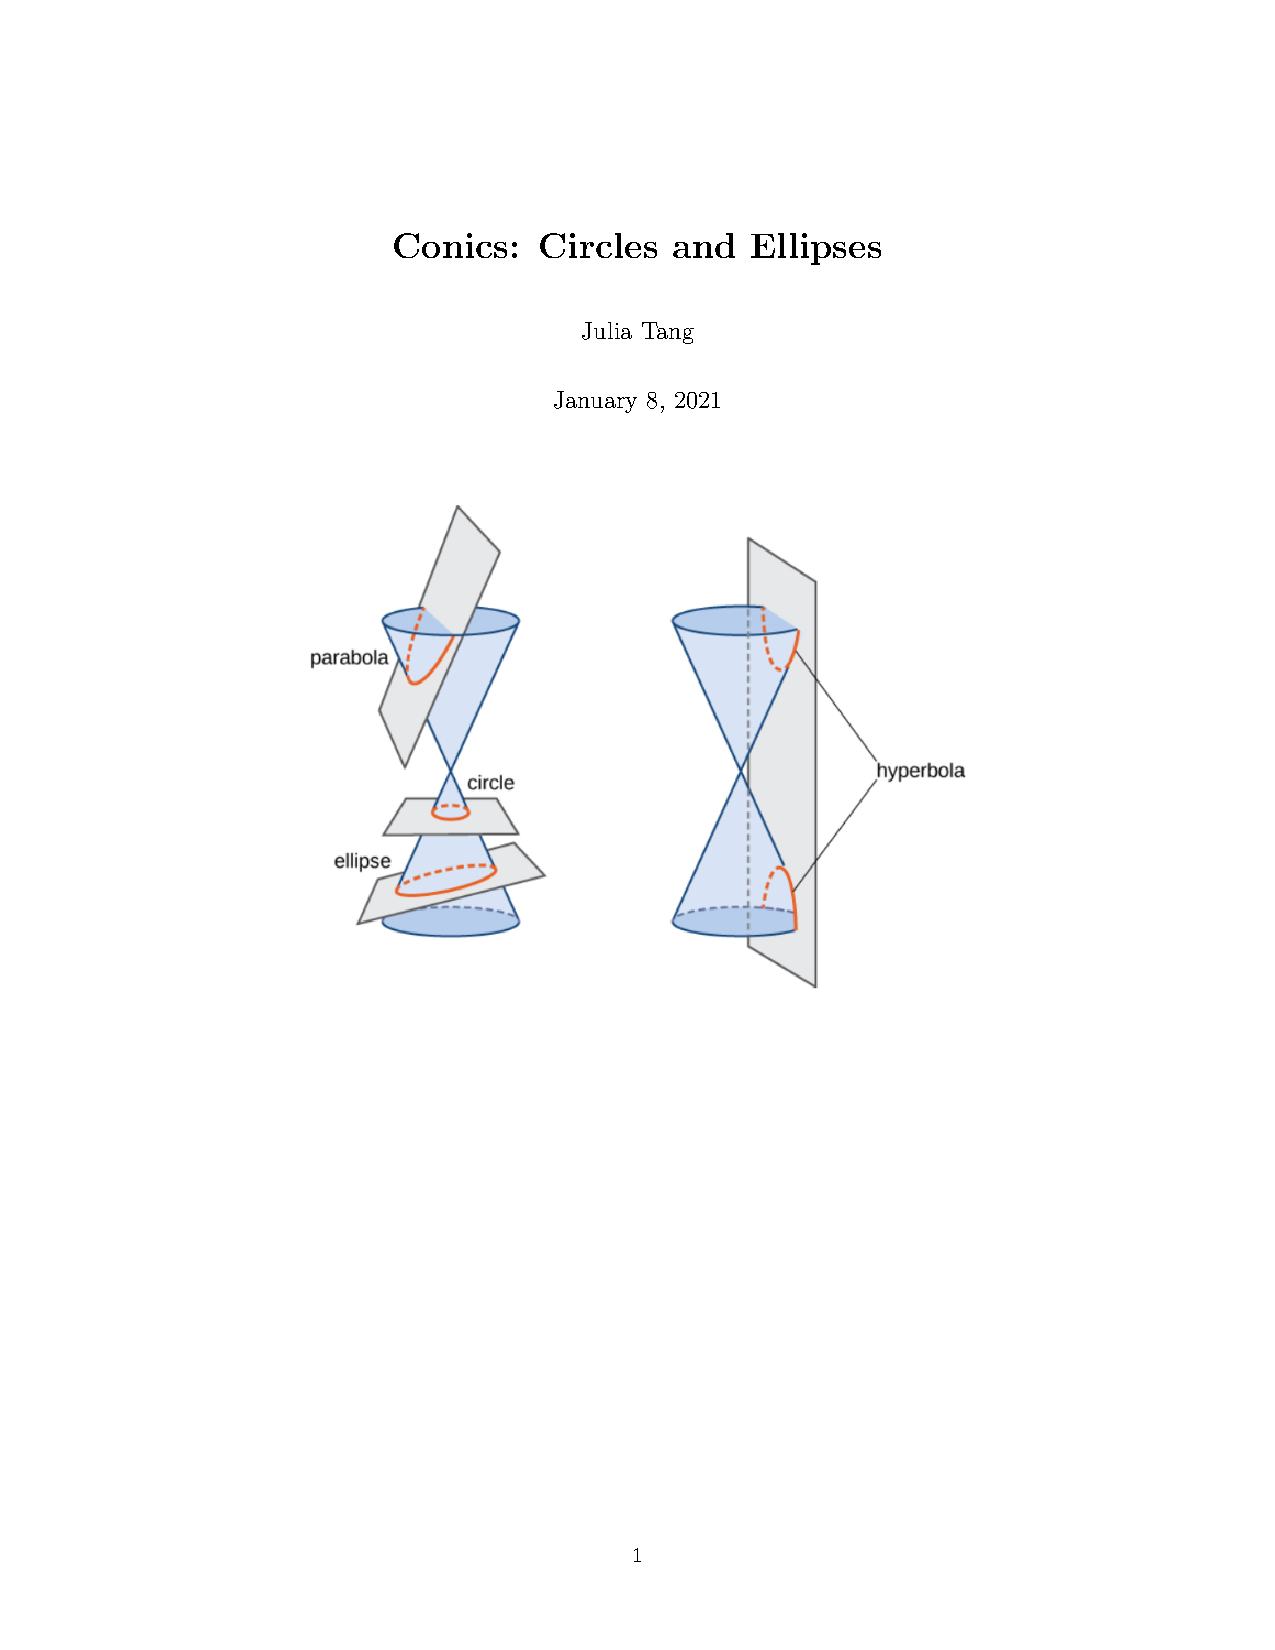
\includegraphics[width=0.7\textwidth]{conics.png}
  \end{center}
\end{figure}
\newpage

\doublespacing
\tableofcontents
\singlespacing

\newpage
\section{Circles and Ellipses}

\subsection{The Ellipse Labelled}

\paragraph{\textbf{DEFINITION}}
An \textit{\colorbox{yellowOrange}{ellipse}} is the set of all points for which the sum of their distances, \textcolor{blueGreen2}{$d_1$} and \textcolor{blueGreen1}{$d_2$}, from two fixed points (the foci, \textcolor{redOrange}{$F\prime$} and \textcolor{redOrange}{$F$}) is constant.

For ellipses with a center $(0,0)$:

\begin{figure}[h!]
  \begin{center}
    %\begin{subfigure}[b]{0.4\linewidth}
    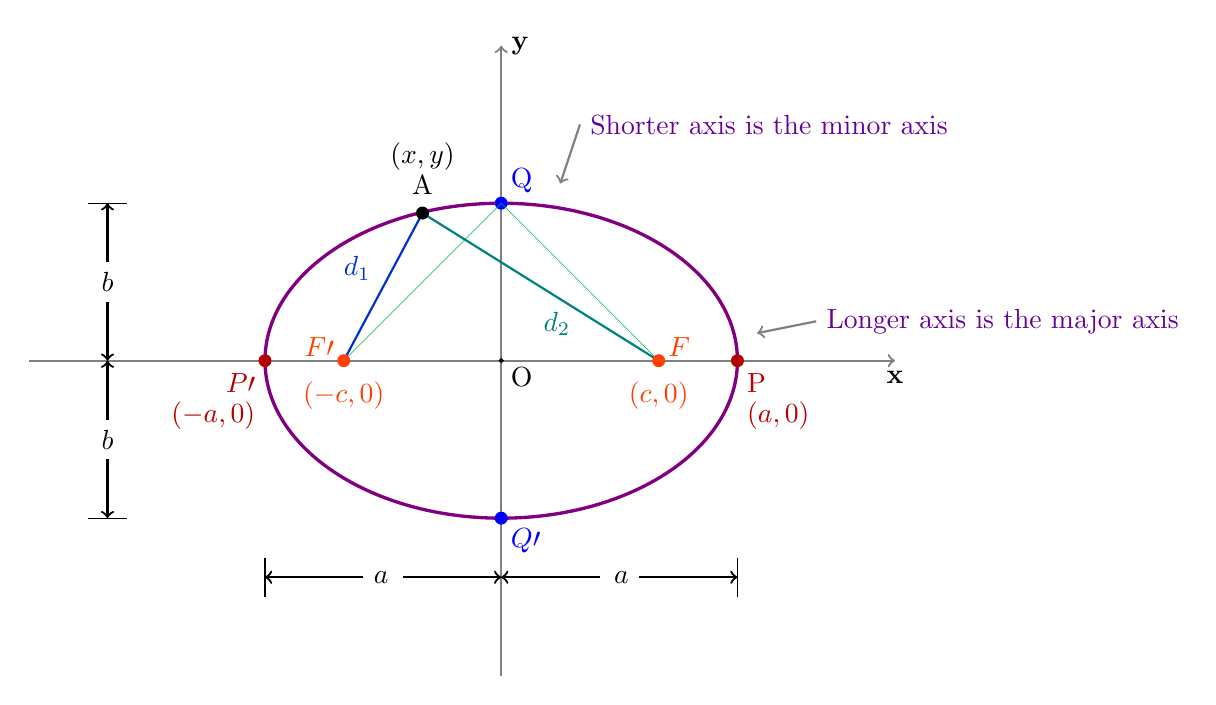
\begin{tikzpicture}
      \draw [->,gray,thick] (0,-4) -- (0,4) node [black,right] {\textbf{y}};
      \draw [->,gray,thick] (-6,0) -- (5,0) node [black,below] {\textbf{x}};
      \draw [blue!50!red,very thick] (0,0) ellipse (3 and 2);
      \draw [black,fill] (0,0) circle [radius=0.025] node [black,below=6,right] {O};
      \draw [blue,fill] (0,2) circle [radius=0.075] node [blue,above=8,right] {Q};
      \draw [<-,gray,thick] (0.75,2.25) -- (1,3) node [red!40!blue,above,right] {Shorter axis is the minor axis};
      \draw [blue,fill] (0,-2) circle [radius=0.075] node [blue,below=8,right] {$Q\prime$};
      \draw [blue!30!green,very thin] (-2,0) -- (0,2);
      \draw [blue!30!green,very thin] (2,0) -- (0,2);
      \draw [black!30!red,fill] (3,0) circle [radius=0.075] node [black!30!red,below=8,right] {P}
      node [black!30!red, below=20,right] {$(a, 0)$};
      \draw [black!30!red,fill] (-3,0) circle [radius=0.075] node [black!30!red,below=8,left] {$P\prime$}
      node [black!30!red, below=20,left] {$(-a, 0)$};
      \draw [<-,gray,thick] (3.25,0.35) -- (4,0.5) node [red!40!blue,above,right] {Longer axis is the major axis};
      \draw [blue!80!green,thick] (-2,0) -- (-1,1.875) node [blue!80!green,below=20,left=15] {$d_1$};
      \draw [blue!50!green,thick] (2,0) -- (-1,1.875) node [blue!50!green,below=40,right=40] {$d_2$};
      \draw [orange!50!red,fill] (2,0) circle [radius=0.075] node [orange!50!red,above=5,right] {$F$}
      node [orange!50!red,below=4] {$(c, 0)$};
      \draw [orange!50!red,fill] (-2,0) circle [radius=0.075] node [orange!50!red,above=5,left] {$F\prime$}
      node [orange!50!red,below=4] {$(-c, 0)$};
      \draw [black,fill] (-1,1.875) circle [radius=0.075] node [black,above=3] {A}
      node [black,above=12] {$(x, y)$};
      \draw [black] (-5.25,2) -- (-4.75,2);
      \draw [<-,black,thick] (-5,0) -- (-5,0.75) node [black,above] {$b$};
      \draw [->,black,thick] (-5,1.25) -- (-5,2);
      \draw [black] (-5.25,-2) -- (-4.75,-2);
      \draw [<-,black,thick] (-5,0) -- (-5,-0.75) node [black,below] {$b$};
      \draw [->,black,thick] (-5,-1.25) -- (-5,-2);
      \draw [black] (-3,-2.5) -- (-3,-3);
      \draw [black] (3,-2.5) -- (3,-3);
      \draw [<-,black,thick] (-3,-2.75) -- (-1.75,-2.75) node [black,right] {$a$};
      \draw [->,black,thick] (-1.25,-2.75) -- (0,-2.75);
      \draw [<-,black,thick] (3,-2.75) -- (1.75,-2.75) node [black,left] {$a$};
      \draw [->,black,thick] (1.25,-2.75) -- (0,-2.75);
    \end{tikzpicture}
  \end{center}
  \caption{The ellipse labelled with its foci, vertices, and components.}
  \label{fig:ellipse1}
\end{figure}
\begin{figure}[H]
  \begin{center}
    \begin{tikzpicture}
      \draw [->,gray,thick] (0,-0.5) -- (0,4) node [black,right] {\textbf{y}};
      \draw [->,gray,thick] (-6,0) -- (5,0) node [black,below] {\textbf{x}};
      \draw [blue,very thick] (-4,0) -- (0,3.5) node [black,below=40,left=50] {$a$};
      \draw [blue,very thick] (4,0) -- (0,3.5) node [black,below=40,right=50] {$a$};
      \draw [green,very thick] (0,0) -- (0,3.5) node [black,below=50,left] {$b$};
      \draw [red,very thick] (-4,0) -- (4,0) node [black,below=15,left=40] {$c$};
      \draw [black,fill] (0,3.5) circle [radius=0.075];
      \draw [black,fill] (-4,0) circle [radius=0.075];
      \draw [black,fill] (4,0) circle [radius=0.075];
      \draw [black,fill] (0,0) circle [radius=0.075];
    \end{tikzpicture}
  \end{center}
  \caption{The a, b, and c components of an ellipse.}
  \label{fig:ellipse2}
\end{figure}

As seen in Figure \ref{fig:ellipse2}, the \colorbox{yellowOrange}{ellipse has an a, b, and c component}. Let the string length be \textcolor{blue}{$2a$}. For ellipses, using Pythagorean Theorem, the equation for any side, given the other two, becomes

\[
\highlight{a^2 = b^2 + c^2}
\]

\subsection{Deriving the Ellipse's Equation}

Using the two distances, \textcolor{blueGreen1}{$d_1$} and \textcolor{blueGreen2}{$d_2$},
\begin{align*}
  d_1 + d_2 = 2a
\end{align*}
\begin{align*}
  \sqrt{(x - c)^2 + (y - 0)}^2 + \sqrt{(x - c)^2 + (y - 0)^2} &= 2a\\
  \sqrt{(x + c)^2 + y^2})^2 &= (2a - \sqrt{(x - c)^2 + y^2})^2\\
  (x + c)^2 + y^2 &= 4a^2 - 4a\sqrt{(x - c)^2 + y^2} + ((x - c)^2 + y^2)\\
  x^2 + 2cx + c^2 + y^2 &= 4a^2 - 4a\sqrt{(x - c)^2 + y^2} + x^2 - 2cx + c^2 + y^2\\
\end{align*}
\begin{flushleft}
  Cancelling like-terms will give you this:
\end{flushleft}
\begin{align*}
  (4a\sqrt{(x - c)^2 + y^2})^2 &= (4a^2 - 4cx)^2
\end{align*}
\begin{flushleft}
\newpage
  Again, cancel like-terms and factor out a four to get
\end{flushleft}
\begin{align*}
  a^2((x - c)^2 + y^2) = a^4 - 2a^2cx + c^2x^2
\end{align*}
\begin{flushleft}
  Further simplification will become
\end{flushleft}
\begin{align*}
  a^2(x^2 - 2cx + c^2 + y^2) &= a^4 - 2a^2cx + c^2x^2\\
  a^2x^2 - 2a^2cx + a^2c^2 + a^2y^2 &= a^4 - 2a^2cx + c^2x^2\\
\end{align*}
\begin{flushleft}
  Cancel like-terms again and you will get
\end{flushleft}
\begin{align*}
  (a^2 - c^2)x^2 + a^2y^2 &= a^4 - a^2c^2\\
  (a^2 - c^2)x^2 + a^2y^2 &= a^2(a^2 - c^2)\\
  \frac{(a^2c^2)x^2}{a^2(a^2 - c^2)} + \frac{a^2y^2}{a^2(a^2 - c^2)} &= 1\\
  \frac{x^2}{a^2} + \frac{y^2}{a^2 - c^2} &= 1
\end{align*}
\begin{flushleft}

  Thus, the \emph{final equation for an ellipse} is:

\end{flushleft}
\begin{align*}
  \highlight{\frac{x^2}{a^2} + \frac{y^2}{b^2} = 1}
\end{align*}

\newpage
\subsection{Ellipse Examples}
\subsubsection{Example 1}
\begin{question}

Graph, locate \textit{foci} and state \textit{eccentricity}

\begin{align*}
  \frac{x^2}{25} + \frac{y^2}{16} = 1
\end{align*}
\end{question}
  \begin{center}
    $a = 5$ and $b = 4$
  \end{center}
\begin{align*}
  a^2 &= b^2 + c^2\\
  25 &= 16 + c^2\\
  9 &= c^2\\
  3 &= c
\end{align*}
\begin{flushleft}
  Now, let's find the eccentricity
\end{flushleft}
\begin{align*}
  e = \frac{c}{a} = \frac{3}{5}
\end{align*}
\begin{flushleft}
  Finally, using the c value, you can calculate where the foci and vertices are.
  Graphing this ellipse will give you:
\end{flushleft}

\begin{figure}[H]
  \begin{center}
    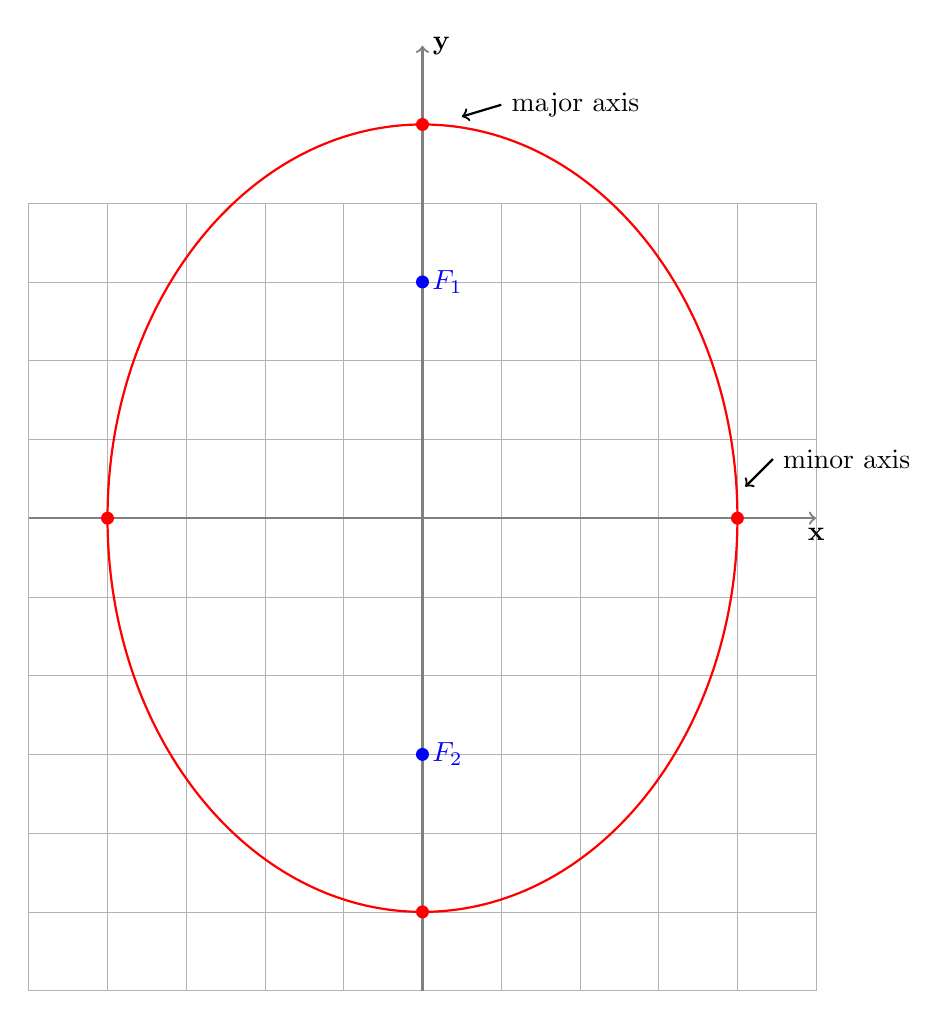
\begin{tikzpicture}
      \draw[step=1cm,white!40!gray,very thin] (-5,-6) grid (5,4);
      \draw [->,gray,thick] (0,-6) -- (0,6) node [black,right] {\textbf{y}};
      \draw [->,gray,thick] (-5,0) -- (5,0) node [black,below] {\textbf{x}};
      \draw [red,thick] (0,0) ellipse (4 and 5);
      \draw [red,fill] (0,5) circle [radius=0.075];
      \draw [red,fill] (0,-5) circle [radius=0.075];
      \draw [red,fill] (4,0) circle [radius=0.075];
      \draw [red,fill] (-4,0) circle [radius=0.075];
      \draw [blue,fill] (0,3) circle [radius=0.075] node [blue,above,right] {$F_1$};
      \draw [blue,fill] (0,-3) circle [radius=0.075] node [blue,above,right] {$F_2$};
      \draw [<-,black,thick] (0.5,5.1) -- (1,5.25) node [black,above,right] {major axis};
      \draw [<-,black,thick] (4.1,0.4) -- (4.45,0.75) node [black,above,right] {minor axis};
    \end{tikzpicture}
  \end{center}
  \caption{The correct graph of this example.}
  \label{fig:ellipse3}
\end{figure}

\newpage
\begin{flushleft}
  \subsection{Ellipses with Center $(h,k)$}

  \paragraph{Standard Forms} For an ellipse centered at $(h, k)$, the standard form is

\begin{align*}
  \highlight{\frac{(x - h)^2}{a^2} + \frac{(y - k)^2}{b^2} = 1}
\end{align*}

i.e., in Figure \ref{fig:ellipse4}, the center of the ellipse and the ellipse's $a$ and $b$ values result in this ellipse:

\end{flushleft}
\begin{figure}[H]
  \begin{center}
    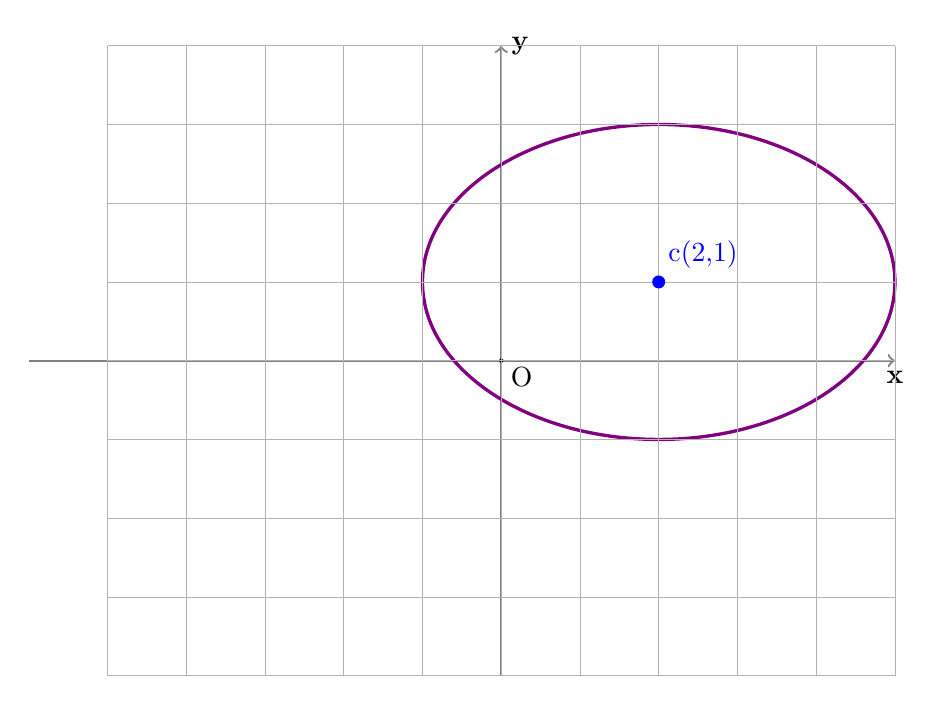
\begin{tikzpicture}
      \draw [->,gray,thick] (0,-4) -- (0,4) node [black,right] {\textbf{y}};
      \draw [->,gray,thick] (-6,0) -- (5,0) node [black,below] {\textbf{x}};
      \draw [blue!50!red,very thick] (2,1) ellipse (3 and 2);
      \draw [black,fill] (0,0) circle [radius=0.025] node [black,below=6,right] {O};
      \draw[step=1cm,white!40!gray,very thin] (-5,-4) grid (5,4);
      \draw [blue,fill] (2,1) circle [radius=0.075] node [blue,above=10,right] {c(2,1)};
    \end{tikzpicture}
  \end{center}
  \caption{An example of an ellipse centered at $(h, k)$.}
  \label{fig:ellipse4}
\end{figure}
\begin{flushleft}

  In Figure \ref{fig:ellipse4}, the $h$ is $2$ and the $k$ is $1$.

\end{flushleft}

\newpage
\begin{flushleft}
  \subsubsection{Example 2 (\textit{An ellipse centered at $(h, k)$)}}
\end{flushleft}

\begin{question}

  Graph, locate \textit{foci} and state \textit{eccentricity}.

  \begin{align*}
    \frac{(x - 1)^2}{16} + \frac{(y + 2)^2}{9} = 1
  \end{align*}
\end{question}
\begin{multicols}{2}
  \begin{align*}
    c(h, k) = (1,-2)
  \end{align*}

  \begin{align*}
    a^2 = 16
  \end{align*}
  \begin{align*}
    b^2 = 9
  \end{align*}
  \begin{align*}
    c^2 = a^2 - b^2
  \end{align*}
  \begin{align*}
    c^2 = 7
  \end{align*}
  \begin{align*}
    c = \sqrt{7}
  \end{align*}

  \begin{align*}
    e = \frac{c}{a} = \frac{\sqrt{7}}{4}
  \end{align*}

  \begin{align*}
    v_1(1 + 4, -2) = (5, -2)
  \end{align*}
  \begin{align*}
    v_2(1 - 4, -2) = (-3, -2)
  \end{align*}

  \begin{align*}
    cv_1(1, -2 + 3) = (1, 1)
  \end{align*}
  \begin{align*}
    cv_2(1, -2 - 3) = (1, -5)
  \end{align*}

  \begin{align*}
    F_1(1 + \sqrt{7}, -2)
  \end{align*}
  \begin{align*}
    F_2(1 - \sqrt{7}, -2)
  \end{align*}
\end{multicols}
\begin{figure}[H]
  \begin{center}
    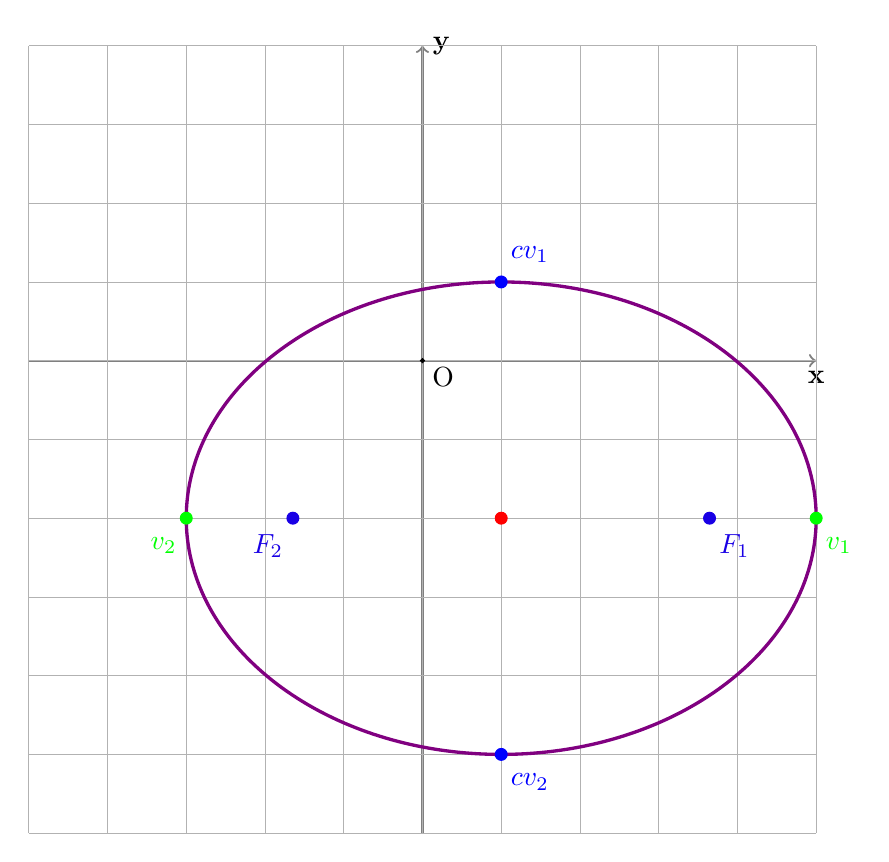
\begin{tikzpicture}
      \draw [->,gray,thick] (0,-6) -- (0,4) node [black,right] {\textbf{y}};
      \draw [->,gray,thick] (-5,0) -- (5,0) node [black,below] {\textbf{x}};
      \draw[step=1cm,white!40!gray,very thin] (-5,-6) grid (5,4);
      \draw [blue!50!red,very thick] (1,-2) ellipse (4 and 3);
      \draw [black,fill] (0,0) circle [radius=0.025] node [black,below=6,right] {O};
      \draw [blue,fill] (1,1) circle [radius=0.075] node [blue,above=10,right] {$cv_1$};
      \draw [blue,fill] (1,-5) circle [radius=0.075] node [blue,below=10,right] {$cv_2$};
      \draw [green,fill] (5,-2) circle [radius=0.075] node [green,below=10,right] {$v_1$};
      \draw [green,fill] (-3,-2) circle [radius=0.075] node [green,below=10,left] {$v_2$};
      \draw [red!10!blue,fill] (3.6457,-2) circle [radius=0.075] node [red!10!blue,below=10,right] {$F_1$};
      \draw [red!10!blue,fill] (-1.6457,-2) circle [radius=0.075] node [red!10!blue,below=10,left] {$F_2$};
      \draw [red,fill] (1,-2) circle [radius=0.075];
    \end{tikzpicture}
  \end{center}
  \caption{The major points and the finished graph of this example.}
  \label{fig:ellipse5}
\end{figure}

\subsection{The Equation of a Circle}
\begin{figure}[H]
  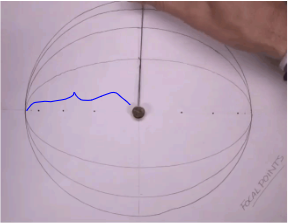
\includegraphics[width=0.7\textwidth,center]{Circle.png}
  \caption{A circle (the radius is blue)}
  \label{fig:circle}
\end{figure}
\begin{center}
  $a = b = r$

  $\frac{(x - h)^2}{r^2} + \frac{(y - k)^2}{r^2} = 1$

  $\highlight{(x - h)^2 + (y - k)^2 = r^2}$
\end{center}

\newpage
\section{Completing the Square}

In some cases, completing the square is necessary to rewrite the given equation into standard form.

For example, a standard polynomial would look as so
\begin{center}
  $x^2 + ax + (\frac{1}{2}a)^2 - (\frac{1}{2}a)^2$
\end{center}
In terms of areas, the green area is what completing the square is finding (literally completing the overall square).
\begin{figure}[H]
  \begin{center}
    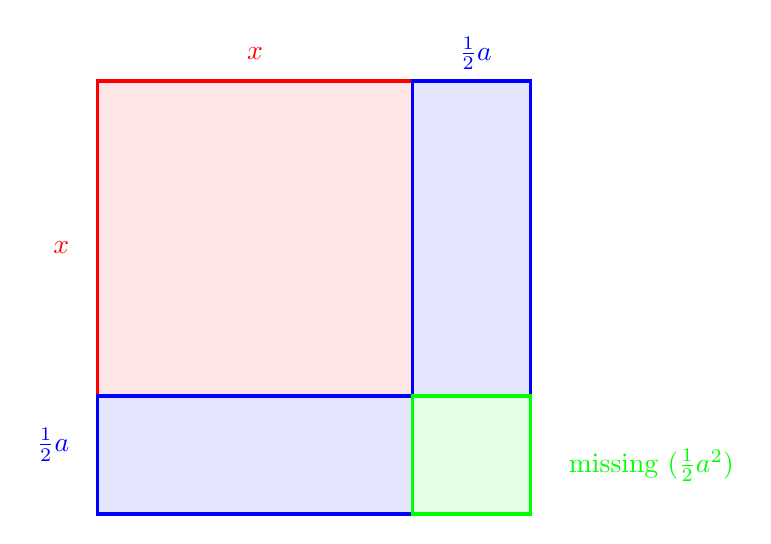
\begin{tikzpicture}
      \filldraw [color=red,fill=red!10,very thick] (0,0) rectangle (4,4) node [red,above=10,left=50] {$x$}
      node [red,below=60,left=120] {$x$};
      \filldraw [color=blue,fill=blue!10,very thick] (4,0) rectangle (5.5,4)
      node [blue,above=10,left=10] {$\frac{1}{2}a$};
      \filldraw [color=blue,fill=blue!10,very thick] (0,0) rectangle (4,-1.5) node [blue,above=25,left=120] {$\frac{1}{2}a$};
      \filldraw [color=green,fill=green!10,very thick] (4,-1.5) rectangle (5.5,0) node [green,below=25,right=10] {missing $(\frac{1}{2}a^2)$};
    \end{tikzpicture}
  \end{center}
  \caption{The polynomial visualized.}
  \label{fig:completingsquare}
\end{figure}

\subsection{Example 3}
\begin{question}
  Convert each equation to standard form by \underline{completing the square} in $x$ and $y$. Graph, locate \textit{foci} and state \textit{eccentricity}.
  \begin{center}
    $9x^2 + 25y^2 - 36x + 50y - 164 = 0$
  \end{center}
\end{question}
\begin{align*}
  (9x^2 - 36x) &+ (25y^2 + 50y) &= 164\\\\
  9(x^2 - 4x + \textcolor{blue}{4}) + 25(y^2 + 2y + \textcolor{red}{1}) &= 164 + \textcolor{blue}{36} + \textcolor{red}{25}\\\\
  \frac{9(x - 2)^2}{225} +\frac{25(y + 1)^2}{225} &= \frac{225}{225}\\\\
  \frac{(x - 2)^2}{36} + \frac{(y + 1)^2}{9} &= 1
\end{align*}

\section{Eccentricity}

Eccentricity is the ``weirdness'' of a circle; for example, a circle's eccentricity is always 0.

For \textit{hyperbolas}, $e\ >\ 1$

    \hspace{1.1cm}\textit{ellipses},   $0\ <\ e\ <\ 1$

    \hspace{1.25cm}\textit{circles},    $e\ =\ 0$

    \hspace{1cm}\textit{parabola},   $e\ =\ 1$

The equation for eccentricity is

\begin{equation*}
  \highlight{e\ =\ \frac{c}{a}}
\end{equation*}

An infinite eccentricity results in a line.

\newpage
\section{Hyperbolas}

\paragraph{DEFINITION} A \emph{hyperbola} is the set of all points where the difference between their distances from two fixed points (the foci) is constant.

\begin{figure}[H]
  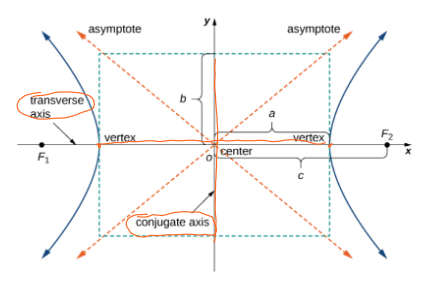
\includegraphics[width=0.7\textwidth,center]{Hyperbola Labelled.png}
  \caption{The different aspects of the hyperbola, labelled.}
  \label{fig:hyperbola1}
\end{figure}

\paragraph{INTRO} $(x, y)$ is an \emph{ellipse} if $d_1 + d_2$ is a constant. However, $(x, y)$ is a \highlight{\textit{hyperbola}} if $|d_1 - d_2|$ is a constant.

\begin{figure}[H]
    \includegraphics[width=0.7\textwidth,center]{Hyperbola and ellipse.png}
    \caption{The top figure is the ellipse while the bottom figure displays how the hyperbola is labelled in comparison. As seen in the figure, one arc of the hyperbola is called a branch.}
    \label{fig:hyperbola2}
\end{figure}
\begin{figure}[H]
  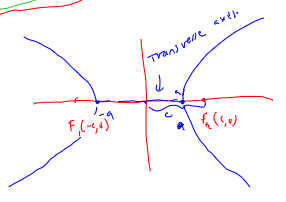
\includegraphics[width=0.5\textwidth,center]{Hyperbola.png}
  \caption{As seen here, the transverse axis is labelled.}
  \label{fig:hyperbola3}
\end{figure}

The transverse axis is the equivalent to an ellipse's major axis; the foci and vertices are located on the axis. Its length is $2a$, so it doesn't extend past the foci.

\subsection{The Hyperbola's Equations}
\subsubsection{Deriving the Hyperbola's Standard Form}

\begin{align*}
  |d_1 &- d_2| = 2a\\
  \sqrt{(x + c)^2 + (y - 0)^2} &- \sqrt{(x - c)^2 + (y)^2} = 2a\\
  &.\\
  &.\\
  &.
\end{align*}
\begin{equation*}
  \highlight{\frac{x^2}{a^2} - \frac{y^2}{b^2} = 1}
\end{equation*}

In the hyperbola's case,

\begin{equation*}
  \highlight{b^2 = c^2 - a^2}
\end{equation*}

\subsection{The Elements of a Hyperbola}
\paragraph{What is the significance of b \textit{in} $(b^2 = c^2 - a^2)$}?

Rearranging the standard form of a hyperbola,

\begin{align*}
  \frac{x^2}{a^2} &- \frac{y^2}{b^2} = 1\\
  \frac{y^2}{b^2} &= \frac{x^2}{a^2} - 1\\
  \frac{y^2}{b^2} &= \frac{x^2}{a^2}(1 - \frac{a^2}{x^2})
\end{align*}

You will get this. As $x \rightarrow \infty$, the behavior of $(1 - \frac{a^2}{x^2})$ will approach $0$.

Then, the equation will start to look like

\begin{align*}
  \frac{y^2}{b^2} &= \frac{x^2}{a^2}\\
  y^2 &= \frac{b^2}{a^2}x^2\\
\end{align*}
\begin{equation*}
  \highlight{y \pm \frac{b}{a}x}
\end{equation*}

Which is the equation for both asymptote lines in a hyperbola.

\subsection{Example 1}

\begin{question}
  Use the \underline{vertices} and asymptotes to graph the hyperbola. Locate the \textit{\underline{foci}}, find the \underline{equation of the asymptotes}, and state \textit{eccentricity}.
    \begin{center}
      $\frac{x^2}{9} - \frac{y^2}{25} = 1$
    \end{center}
\end{question}
\begin{align*}
  a^2 &= 9           &         &c(0,\ 0)\\
  b^2 &= 25          &         &v_1(0 + a,\ 0) = (3,\ 0)\\
  c^2 &= a^2 + b^2   &         &v_2(0 - a,\ 0) = (-3,\ 0)\\
  c^2 &= 34          &         &cv_1(0,\ 0 + 5) = (0,\ 5)\\
  c &= \sqrt{34}     &         &cv_2(0,\ 0 - 5) = (0,\ -5)
\end{align*}
\begin{align*}
  &F_1(0 + \sqrt{34},\ 0) = (\sqrt{34},\ 0)           &           y = \frac{5}{3}x\\
  &F_2(0 - \sqrt{34},\ 0) = (-\sqrt{34},\ 0)          &           y = \frac{-5}{3}x\\
  &e\ =\ \frac{c}{a}\ =\ \frac{\sqrt{34}}{3}
\end{align*}
\begin{figure}[H]
  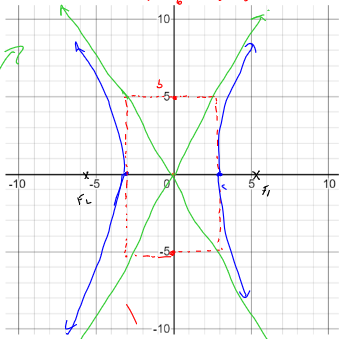
\includegraphics[width=0.7\textwidth,center]{hyperbola1.png}
  \caption{The correct graph of example 1.}
  \label{fig:hyperbola4}
\end{figure}

\newpage
\section{Parabolas}

\paragraph{DEFINITION} A \highlight{parabola} is the set of all points whose distance from a fixed point, called the focus, is equal to the distance from a fixed line, called the \highlight{directrix}. The point halfway between the focus and directrix is called the vertex of the parabola.

\begin{figure}[H]
  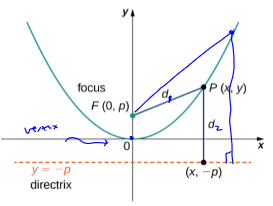
\includegraphics[width=0.7\textwidth,center]{Parabola.png}
  \caption{The different components of the parabola labelled.}
  \label{fig:parabola1}
\end{figure}

\subsection{Deriving the Parabola's Equation}

Given $F(0,\ P)$ and $y\ =\ -P$,

\begin{align*}
  &d_1\ =\ \sqrt{(x\ -\ 0)^2\ +\ (y\ -\ P)^2}\\
  &d_2\ =\ (y\ -\ (-P))\ =\ y\ +\ P
\end{align*}
\begin{align*}
  d_1\ &=\ d_2\\
  \sqrt{(x\ -\ 0)^2\ +\ (y\ -\ P)^2}\ &=\ y\ +\ P\\
  x^2\ +\ (y\ -\ P)^2\ &=\ (y\ +\ P)^2\\
  x^2\ +\ y^2\ -\ 2Py\ +\ P^2\ &=\ y^2\ +\ 2Py\ +\ P^2
\end{align*}

Cancelling the terms $y^2$ and $P^2$, the resulting equation for a parabola centered at $(0\ ,\ 0)$ is

\begin{equation*}
  \highlight{x^2\ =\ 4Py}
\end{equation*}

Here, $|P|$ is the distance from vertex to focus or directrix.

However, if the vertex were at $(h\ ,\ k)$, then the equation for the standard form would be

\begin{equation*}
  \highlight{(x\ -\ h)^2\ =\ 4P(y\ -\ k)}
\end{equation*}
\begin{center}
  or
\end{center}
\begin{equation*}
  \highlight{(y\ -\ k)^2\ =\ 4P(x\ -\ h)}
\end{equation*}

\subsection{Example 1}

\begin{question}
  Find the foci and equation of the \emph{directrix} for this parabola:
  \begin{Center}
    $y^2\ =\ 12x$
  \end{Center}
\end{question}

\begin{align*}
  (y\ -\ 0)^2\ &=\ 4P(x\ -\ 0)\\
  v(0&,\ 0)\\
  4P\ &=\ 12\\
  P\ &=\ 3\\
  F(0\ +\ P,\ 0)\ &=\ (3,\ 0)\\
  directrix:\ x\ &=\ P\ =\ -3
\end{align*}
\begin{figure}[H]
  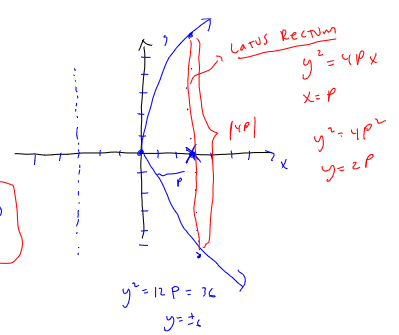
\includegraphics[width=0.7\textwidth,center]{parabola 1.png}
  \caption{The correct graph of this problem.}
  \label{fig:parabola2}
\end{figure}

\subsection{Latus Rectum}

\paragraph{DEFINITION} The Latus Rectum of a parabola is the line segment that passes through the foci, and it is parallel to the directrix. It is labelled in Figure \ref{fig:parabola2}.

\newpage
\subsection{Rotation of Axes}

Here is the commonly seen polynomial:

\begin{equation*}
  Ax^2\ +\ Bxy\ +\ Cy^2\ +\ Dx\ +\ Ey\ +\ F\ =\ 0
\end{equation*}

This is a second degree polynomial. Each constant is denoted by $A$, $B$, $C$, etc. The \highlight{\textbf{cross-term}} is the term \highlight{$Bxy$}.

\subsubsection{Discriminant Test}

The quadratic curve $Ax^2\ +\ Bxy\ +\ Cy^2\ +\ Dx\ +\ Ey\ +\ F\ =\ 0\ $ is

\renewcommand{\theenumi}{\Roman{enumi}}
\begin{justify}
  \begin{enumerate}
     \item a \highlight{parabola} if $B^2\ -\ 4AC\ =\ 0$
     \item an \highlight{ellipse} if $B^2\ -\ 4AC\ <\ 0$
     \item a \highlight{hyperbola} if $B^2\ -\ 5AC\ >\ 0$
  \end{enumerate}
\end{justify}

\end{document}
